\chapter{Zadatak E} \label{ch:e}

U ovom poglavlju je opisan i odrađen zadatak E.

\section{Opis zadatka} \label{sec:e:opis}
na temelju podataka iz d) dijela zadatka, potrebno je odrediti mehaničku snagu koju vozilo mora
utrošiti kako bi prevalilo zadanu rutu sa zadanim profilom vožnje, mehaničku snagu koju vozilo može
iskoristiti na zadanoj rutu sa zadanim profilom vožnje za regeneraciju energije. Potrebno je prikazati
krivulje svake komponente mehaničke snage zasebno i sve na jednom grafu s točno naznačenim
oznakama. Dodatno, za svaku komponentu snage je potrebno odrediti minimalnu, maksimalnu i
srednju vrijednost krivulje, te prikazati je u tabličnom obliku

\section{Rješenje} \label{sec:e:rjesenje}
Prvo je potrebno izračunati apsolutne snage iz zadatka d. To je napravljeno tako da se sve negativne
vrijednosti pretvore u pozitivne. Za regenerativne snage je potrebno oduzeti apsolutne snage od početnih.

\begin{figure}
    \centering
    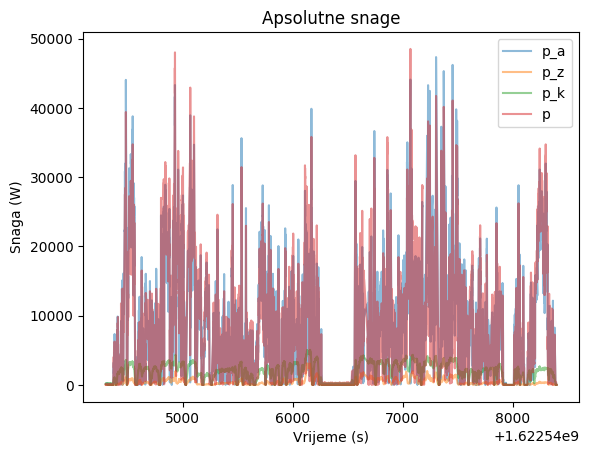
\includegraphics[width=0.8\textwidth]{images/abs_powes.png}
    \caption{Prikaz izračunate apsolutne snage kroz vrijeme.}
    \label{fig:e:abs_power_graph}
\end{figure}

\begin{figure}
    \centering
    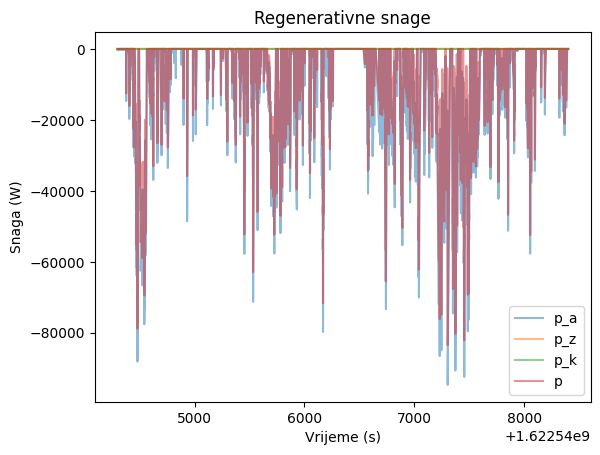
\includegraphics[width=0.8\textwidth]{images/regen_powers.png}
    \caption{Prikaz izračunate regenerativne snage kroz vrijeme.}
    \label{fig:e:regen_power_graph}
\end{figure}


\begin{table}[!ht]
    \centering
    \caption{Anaiza apsolutnih snaga na vozilu}
    \begin{tabular}{lllll}
    \hline
        \textbf{describe} & \textbf{p\_a} & \textbf{p\_z} & \textbf{p\_k} & \textbf{p} \\ \hline
        """count""" & 9776.0 & 9776.0 & 9776.0 & 9776.0 \\ 
        """null\_count""" & 0.0 & 0.0 & 0.0 & 0.0 \\ 
        """mean""" & 6968.339474 & 414.467539 & 1876.065364 & 7304.462425 \\ 
        """std""" & 7581.496918 & 520.405078 & 1315.56626 & 7994.144607 \\ 
        """min""" & 0.0 & 0.0 & 0.0 & 0.0 \\ 
        """25\%""" & 261.422895 & 0.256285 & 216.047435 & 321.075536 \\ 
        """50\%""" & 4894.030421 & 245.45779 & 2122.481816 & 5085.982462 \\ 
        """75\%""" & 10762.063021 & 671.446613 & 2962.317587 & 10817.709694 \\ 
        """max""" & 47349.443215 & 3118.223036 & 5060.441445 & 48529.830356 \\ \hline
    \end{tabular}
    \label{table:c:abs_powers}
\end{table}

\begin{table}[!ht]
    \centering
    \caption{Anaiza regenerativnih snaga na vozilu}
    \begin{tabular}{lllll}
    \hline
        \textbf{describe} & \textbf{p\_a} & \textbf{p\_z} & \textbf{p\_k} & \textbf{p} \\ \hline
        """count""" & 9776.0 & 9776.0 & 9776.0 & 9776.0 \\ 
        """null\_count""" & 0.0 & 0.0 & 0.0 & 0.0 \\ 
        """mean""" & -6451.586294 & 0.0 & 0.0 & -4497.176342 \\ 
        """std""" & 12574.648658 & 0.0 & 0.0 & 10209.126977 \\ 
        """min""" & -94698.88643 & 0.0 & 0.0 & -83475.775983 \\ 
        """25\%""" & -8185.905362 & 0.0 & 0.0 & -2970.0864 \\ 
        """50\%""" & 0.0 & 0.0 & 0.0 & 0.0 \\ 
        """75\%""" & 0.0 & 0.0 & 0.0 & 0.0 \\ 
        """max""" & -0.0 & 0.0 & 0.0 & 0.0 \\ \hline
    \end{tabular}
    \label{table:c:regen_powers}
\end{table}